{
  \definecolor{TempBackground}{RGB}{29, 30, 34}%
  \setbeamercolor{background canvas}{bg = TempBackground}%
  \begin{frame}

    \begin{tikzpicture}[remember picture,overlay]
      \node<1,3->[at=(current page.center)] {%
        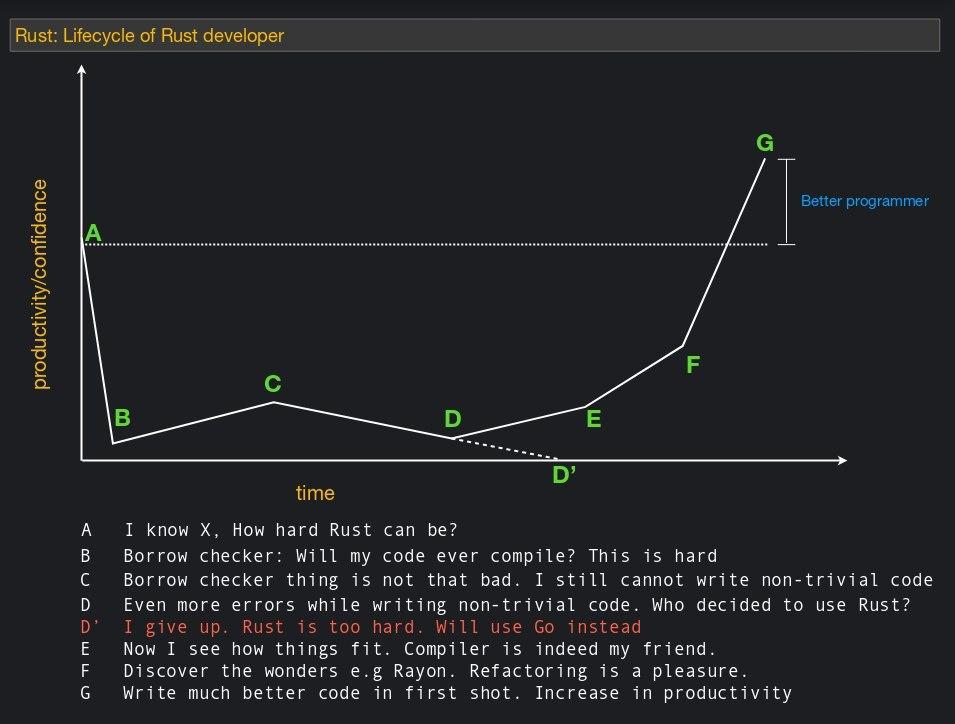
\includegraphics[keepaspectratio,%
        width=\paperwidth,%
        height=\paperheight]{learning_curve.jpg} };

      \node<2>[at=(current page.center)] {%
        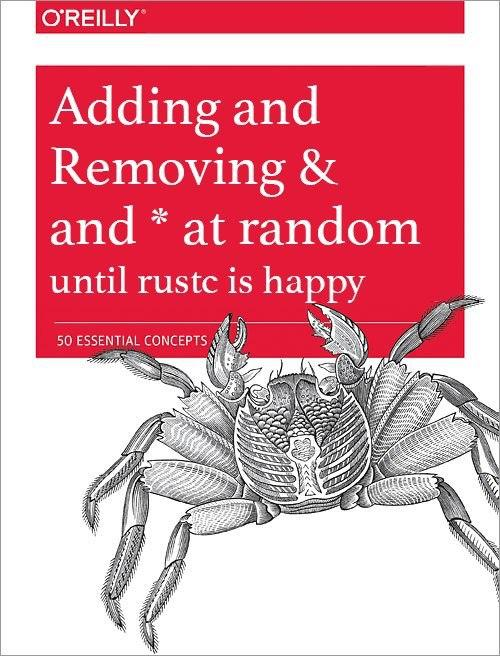
\includegraphics[keepaspectratio,%
        width=\paperwidth,%
        height=\paperheight]{rustc_happy.jpg} };
    \end{tikzpicture}

    \note<1>{

      Изучать Rust \textbf{не так просто}, как другие языки. Сравнить кривую
      обучения можно, пожалуй \textbf{с тем же C++}.

      Данный график полностью отражает \textbf{кривую моего обучения}.

      \begin{itemize}
      \item Прежде, чем изучать Rust, я почитал немного Rust book, \textbf{я
          знал для чего этот язык} предназначен и зачем он мне.
      \item Затем я столкнулся с тем фактом, что сложнее hello world я не могу
        ничего написать, \textbf{компилятор в бешенстве}. Я \textbf{не понимаю,
          что ему надо}.
      \item \textbf{Методом проб и ошибок} я начинаю понимать, что и куда
        писать, чтобы код работал. Это выглядело примерно так ---
        \textbf{следующий слайд!}
      \end{itemize}
    }

    \note<2>{

      Также пытаюсь расставить время жизни объектов наобум, как советует
      компилятор.

    }

    \note<3>{

      \begin{itemize}
      \item Как только я пытаюсь написать какой-то нетривиальный код --- я снова
        в заложниках у компилятора. \textbf{Тут обычно люди и уходят} с Rust.
      \item Я \textbf{начинаю понимать, что компилятор реально от меня хочет},
        что я делаю не так. Я начинаю строить абстракции заранее так, как этого
        хочет компилятор.
      \item Начинают \textbf{познавать что-то новое}: библиотеки, инструменты,
        другие подходы, парадигмы.
      \item Если понимаю архитектуру, то пишу код \textbf{с первого раза верно},
        \textbf{увеличилась производительность} как программиста.
      \end{itemize}

      \textbf{После того, как изучил Rust}, когда пишешь \textbf{на другом
        языке}, всё равно \textbf{пытаешься думать правильно}, составлять
      \textbf{абстракции верно} изначально, невольно \textbf{избегаешь ошибок}
      при работе с памятью!

      \textbf{Кривая похожа на Emacs} --- сначала, вроде, всё легко, потом
      сложно, а потом много нового.

    }

  \end{frame}
}